\chapter{\textbf{Component Diagram And Sequence Diagrams}}

The diagram of the components allowed us to divide our system in different parts each of
them is characterized by an high cohesion. First we listed the components linked to the macro functions described by use cases then we added other micro components thanks to the detailed version of our use cases.
After that we created the Sequence Diagrams and sometimes we refined our Component\\ Diagram bacause of some demands arising from Sequence Diagrams.\\

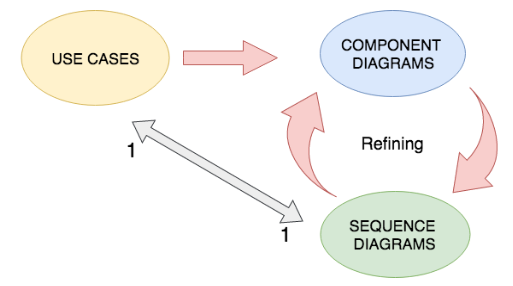
\includegraphics {image.png}
\captionof{figure}{Component - Sequence}

\bigskip The model was created through design tool: MagicDraw. It has allowed us to maintain
consistency in the model between the various diagrams.
